{
\begin{figure}
    \centering
    % \begin{subfigure}[t]{0.3\textwidth}
    %     \centering
    %     \begin{tikzpicture}[xscale=0.8, yscale=-0.35]
    %         \draw [->] (0,0) -- (0,0.5);
    %         \draw [->] (2,0) -- (2,0.5);
    %         \draw (-0.5,0.5) rectangle (2.5,1.5) node[pos=0.5] {$L$};
    %         \draw [->] (0,1.5) -- (0,2);
    %         \draw (-0.3,2) rectangle (0.3,3) node[pos=0.5] {$B$};
    %         \draw [->] (2,1.5) -- (2,2);
    %         \draw (1.7,2) rectangle (2.3,3) node[pos=0.5] {$B$};
    %         \draw [->] (0,3) -- (0,3.5);
    %         \draw (-0.3,3.5) rectangle (0.3,4.5) node[pos=0.5] {$\mathcal{I}$};
    %         \draw [->] (0,4.5) -- (0,5);
    %         \draw (0,5.2) ellipse (0.0875 and 0.2);
    %         \draw (0,5) -- (0,5.4);
    %         \draw (-0.0875,5.2) -- (0.0875,5.2);
    %         \draw (2,3) -- (2,5.2);
    %         \draw [->] (2,5.2) -- (1.3,5.2);
    %         \draw (0.7,4.7) rectangle (1.3,5.7) node[pos=0.5] {$\mathcal{I}$};
    %         \draw [->] (0.7,5.2) -- (0.0875,5.2);
    %         \draw [->] (0,5.4) -- (0,5.9);
    %         \draw [->] (2,5.2) -- (2,5.9);
    %     \end{tikzpicture}
    % \end{subfigure}
    \begin{subfigure}[t]{0.45\textwidth}
        \centering
        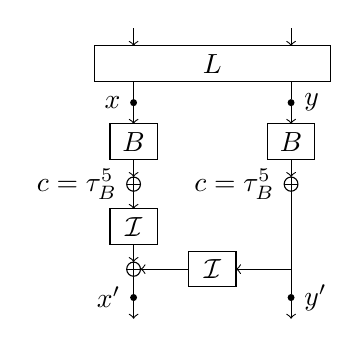
\begin{tikzpicture}[xscale=1.0, yscale=-0.45]
            \draw [->] (0,0) -- (0,0.5);
            \draw [->] (2,0) -- (2,0.5);
            \draw (-0.5,0.5) rectangle (2.5,1.5) node[pos=0.5] {$L$};
            \draw (0,1.5) -- (0,2);
            \fill[black] (0,2.1) ellipse (0.04375 and 0.1);
            \draw (-0.04375,2.1) node[anchor=east] {$x$};
            \draw (2,1.5) -- (2,2);
            \fill[black] (2,2.1) ellipse (0.04375 and 0.1);
            \draw (2.04375,2.1) node[anchor=west] {$y$};
            \draw [->] (0,2.2) -- (0,2.7);
            \draw (-0.3,2.7) rectangle (0.3,3.7) node[pos=0.5] {$B$};
            \draw [->] (2,2.2) -- (2,2.7);
            \draw (1.7,2.7) rectangle (2.3,3.7) node[pos=0.5] {$B$};
            \draw [->] (0,3.7) -- (0,4.2);
            \draw (0,4.4) ellipse (0.0875 and 0.2);
            \draw (0,4.2) -- (0,4.6);
            \draw (-0.0875,4.4) -- (0.0875,4.4);
            \draw (-0.0875,4.4) node[anchor=east] {$c=\tau_B^5$};
            \draw [->] (2,3.7) -- (2,4.2);
            \draw (2,4.4) ellipse (0.0875 and 0.2);
            \draw (2,4.2) -- (2,4.6);
            \draw (1.9125,4.4) -- (2.0875,4.4);
            \draw (1.9125,4.4) node[anchor=east] {$c=\tau_B^5$};
            \draw [->] (0,4.6) -- (0,5.1);
            \draw (-0.3,5.1) rectangle (0.3,6.1) node[pos=0.5] {$\mathcal{I}$};
            \draw [->] (0,6.1) -- (0,6.6);
            \draw (0,6.8) ellipse (0.0875 and 0.2);
            \draw (0,6.6) -- (0,7);
            \draw (-0.0875,6.8) -- (0.0875,6.8);
            \draw (2,4.6) -- (2,6.8);
            \draw [->] (2,6.8) -- (1.3,6.8);
            \draw (0.7,6.3) rectangle (1.3,7.3) node[pos=0.5] {$\mathcal{I}$};
            \draw [->] (0.7,6.8) -- (0.0875,6.8);
            \draw (0,7) -- (0,7.5);
            \fill[black] (0,7.6) ellipse (0.04375 and 0.1);
            \draw (-0.04375,7.6) node[anchor=east] {$x'$};
            \draw (2,6.8) -- (2,7.5);
            \fill[black] (2,7.6) ellipse (0.04375 and 0.1);
            \draw (2.04375,7.6) node[anchor=west] {$y'$};
            \draw [->] (0,7.7) -- (0,8.2);
            \draw [->] (2,7.7) -- (2,8.2);
        \end{tikzpicture}
    \end{subfigure}
    \begin{subfigure}[t]{0.45\textwidth}
        \centering
        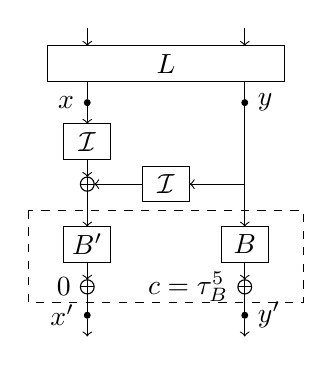
\begin{tikzpicture}[xscale=1.0,yscale=-0.45]
                \draw[->] (0.0,0.0) -- (0.0,0.5);
                \draw[->] (2.0,0.0) -- (2.0,0.5);
                \draw (-0.5,0.5) rectangle (2.5,1.5) node[pos=0.5] {$L$};
                \draw (0.0,1.5) -- (0.0,2.0);
                \fill[black] (0.0,2.1) ellipse (0.04375 and 0.1);
                \draw (-0.04375,2.1) node[anchor=east] {$x$};
                \draw (2.0,1.5) -- (2.0,2.0);
                \fill[black] (2.0,2.1) ellipse (0.04375 and 0.1);
                \draw (2.04375,2.1) node[anchor=west] {$y$};
                \draw[->] (0.0,2.2) -- (0.0,2.7);
                \draw (-0.3,2.7) rectangle (0.3,3.7) node[pos=0.5] {$\mathcal{I}$};
                \draw[->] (0.0,3.7) -- (0.0,4.2);
                \draw (0.0,4.4) ellipse (0.0875 and 0.2);
                \draw (0.0,4.2) -- (0.0,4.6);
                \draw (-0.0875,4.4) -- (0.0875,4.4);
                \draw (2.0,2.2) -- (2.0,4.4);
                \draw[->] (2.0,4.4) -- (1.3,4.4);
                \draw (0.7,3.9) rectangle (1.3,4.9) node[pos=0.5] {$\mathcal{I}$};
                \draw[->] (0.7,4.4) -- (0.0875,4.4);
                \draw[->] (0.0,4.6) -- (0.0,5.6);
                \draw (-0.3,5.6) rectangle (0.3,6.6) node[pos=0.5] {$B'$};
                \draw[->] (2.0,4.4) -- (2.0,5.6);
                \draw (1.7,5.6) rectangle (2.3,6.6) node[pos=0.5] {$B$};
                \draw[->] (0.0,6.6) -- (0.0,7.1);
                \draw (0.0,7.3) ellipse (0.0875 and 0.2);
                \draw (0.0,7.1) -- (0.0,7.5);
                \draw (-0.0875,7.3) -- (0.0875,7.3);
                \draw (-0.0875,7.3) node[anchor=east] {$0$};
                \draw[->] (2.0,6.6) -- (2.0,7.1);
                \draw (2.0,7.3) ellipse (0.0875 and 0.2);
                \draw (2.0,7.1) -- (2.0,7.5);
                \draw (1.9125,7.3) -- (2.0875,7.3);
                \draw (1.9125,7.3) node[anchor=east] {$c=\tau_B^5$};
                \draw[dashed] (-0.75,5.15) rectangle (2.75,7.75);
                \draw (0.0,7.5) -- (0.0,8.0);
                \fill[black] (0.0,8.1) ellipse (0.04375 and 0.1);
                \draw (-0.04375,8.1) node[anchor=east] {$x'$};
                \draw (2.0,7.5) -- (2.0,8.0);
                \fill[black] (2.0,8.1) ellipse (0.04375 and 0.1);
                \draw (2.04375,8.1) node[anchor=west] {$y'$};
                \draw[->] (0.0,8.2) -- (0.0,8.7);
                \draw[->] (2.0,8.2) -- (2.0,8.7);
        \end{tikzpicture}
    \end{subfigure}
    \FigDef{propagation-affine-bottom}{Propagation of affine mappings through the inverses. The dashed area contains the outer affine parts.}
\end{figure}
}